\documentclass{ReportTemplate}


\title{CSEL}
\author{Macherel Rémy}
\date{\today}
\subtitle{Rapports des TP}
\subsubtitle{}
\location{Fribourg,}
\contact{remy.macherel@master.hes-so.ch}
\version{1.0}



\begin{document}
\maketitlepage

\newpage

\maketableofcontent

\medskip
\chapter{TP 1}
\section{Résumé du travail pratique 1}
Dans ce TP, nous allons mettre en place un environnement de développement afin de faciliter les développements futures. Cet environnement utilise des container Docker (Docker-compose) pour assurer la compatibilité entre les différentes machines. Un container est composé de tous les outils nécessaire à la cross-compilation et l'autre pour la mise en place d'une partition réseau SAMBA afin de partager facilement les programmes cross-compilés avec le NanoPi.

\section{Réponses aux questions}
\subsection{Comment faut-il procéder pour générer le U-Boot ?}
On peut regénérer le u-boot uniquement avec la commande : make uboot-rebuild\newline
See : https://github.com/ARM-software/u-boot/blob/master/Makefile \newline
--> TODO : Ajouter 5-6 lignes qui expliquent ce que fais le make de U-Boot
\subsection{Comment peut-on ajouter et générer un package supplémentaire dans le Buildroot ?}
e ne comprends pas trop le sens de la question mais au sens général, il faut ajouter le binaire ainsi que des fichiers de configurations (qui définissent par exemple les dépendances).
On peut par exemple importer depuis GitLab automatiquement un packet, ou encore ajouter des paquet pour le user space ou le kernel space et tout cela change les étapes a effectuer. 
Pour plus d'informations, la section 18 de la \href{https://buildroot.org/downloads/manual/manual.html#adding-packages}{documentation}.

\subsection{Comment doit-on procéder pour modifier la configuration du noyau Linux ?}
La commande make linux-menuconfig permet de configurer le noyau et on peut ensuite ajouter/enlever des modules du noyaux et finalement faire make linux-rebuild afin de reconstruire le noyau.
\newpage
\subsection{Comment faut-il faire pour générer son propre rootfs ?}
Comme c'est Buildroot qui s'occupe de générer le Rootfs, c'est lui qu'il faut configurer \newline
cd /buildroot \newline
make menuconfig \newline
On peut aussi par exemple modifier le skelette utilisé pour modifier la structure des dossiers du rootfs.
On peut aussi ajouter des fichiers/scripts/dossiers par défaut dans le rootfs en ajoutant un rootfs\_overlay \textit{/buildroot/board/friendlyarm/nanopi-neo-plus2/rootfs\_overlay/}. 
Ils seront automatiquement inséré dans le rootfs après chaques générations.

\subsection{Comment faudrait-il procéder pour utiliser la carte eMMC en lieu et place de la carte SD ?}
Il faut commencer par modifier le script de démarrage en modifiant les deux lignes suivantes. Il faut remplacer le \textbf{0} par le numéro de MMC que l'on veut : \newline
 fatload mmc \textbf{0} \$kernel\_addr\_r\ Image \newline
 fatload mmc \textbf{0} \$fdt\_addr\_r nanopi-neo-plus2.dtb \newline
On peut avoir des informations sur les mmc disponible en interrompant le U-Boot et en tappant la commande : \newline
\begin{minted}{shell}
    => mmc list
    mmc@1c0f000: 0 (SD) 
    mmc@1c10000: 2 
    mmc@1c11000: 1 
\end{minted}

Il faut ensuite recompiler le script avec la commande make et reflasher la carte. Enfin il ne faut pas oublier également de charger l'Image et le device tree depuis la carte SD vers la mmc interne (a faire une seul fois) ainsi que de modifier le script de démarrage pour utiliser celui que l'on vient de compiler avec la commande : \newline
\begin{minted}{shell}
    setenv boot_scripts boot.cifs
\end{minted}
 
Finalement, on peut sauvegarder les modifications avec la commande :\newline
\begin{minted}{shell}
    saveenv
\end{minted}
\subsection{Dans le support de cours, on trouve différentes configurations de l’environnement de développement. Qu’elle serait la configuration optimale pour le développement uniquement d’applications en espace utilisateur ?}
Si on développe uniquement dans le userspace, on pourrait imaginer que l'on flash la eMMC comme décrit à la question précédente pour s'affranchir de carte SD et qu'on développe sur notre ordinateur.
Pour le partage des programmes une partition NFS ou la partition CIFS sont très bien et permettent de rendre transparent le transfert des programmes.

\section{Synthèse des connaissances acquises}
\subsection{Non acquis}
Aucune
\subsection{Acquis, mais à exercer}
Les Makefile
\subsection{Parfaitement acquis}
Tout le reste (déjà globalement vu dans un cours précédent)
\section{Infos utiles à retenir}
Pour monter automatiquement un disque réseau cifs : \newline
\begin{minted}[fontsize=\tiny]{shell}
echo "//<server_ip>/workspace /workspace cifs username=<username>, password=<password>,port=1445,noserverino" >> /etc/fstab
\end{minted}
Lorsqu'on créer une nouvelle partition, il faut l'aligner sur 2048 bits. On peut calculer le début de la prochaine partition par rapport à la précédente comme ceci : \newline
<prev\_end\_sector> + (2048 - <prev\_end\_sector>  \% 2048)\newline
\section{Feedback global}
Dans l'ensemble laboratoire très intéressant. Assez dirigé pour nous indiquer la bonne voie mais pas trop pour qu'on puisse tester des choses.
Nous aurions bien souhaité un peu plus de maitère sur les Makefiles.
\chapter{TP 2}
\section{Réponses aux questions}
\subsection{Trouvez la signification des 4 valeurs affichées lorsque l’on tape la commande cat /proc/sys/kernel/printk}
Cela affiche les console\_loglevel (niveaux de logs de la console) actuels, dans notre cas sur le nanopi les valeurs affichées sont 7 4 1 7, comme le montre la \href{https://www.kernel.org/doc/html/latest/core-api/printk-basics.html}{documentation} l'ordre des chiffres correspond à :
\begin{enumerate}
    \item current
    \item default
    \item minimum
    \item boot-time default
\end{enumerate}

\begin{figure}[H]
    \centering
    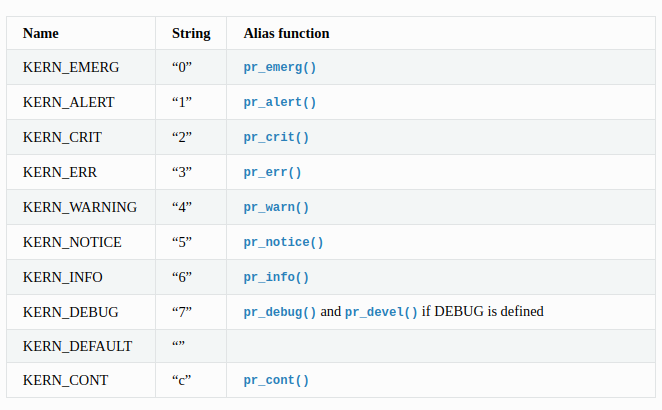
\includegraphics[width=0.7\textwidth]{images/console_loglevels.png}
    \caption{Console log levels correspondance}
    \label{fig:LogLevels}
\end{figure}

\section{Feedback global}

\chapter{TP 3}
\section{Résumé du TP3}
Salut
\end{document}


